%
% This file is part of Calicut University Question Paper Collection.
%
% Copyright (c) 2012-2015 Mohammed Sadik P. K. <sadiq (at) sadiqpk (d0t) org>.
% License: GNU GPLv3 or later
%
% Calicut University Question Paper Collection is free software: you can
% redistribute it and/or modify
% it under the terms of the GNU General Public License as published by
% the Free Software Foundation, either version 3 of the License, or
% (at your option) any later version.
% 
% Calicut University Question Paper Collection is distributed in the hope
% that it will be useful,
% but WITHOUT ANY WARRANTY; without even the implied warranty of
% MERCHANTABILITY or FITNESS FOR A PARTICULAR PURPOSE.  See the
% GNU General Public License for more details.
% 
% You should have received a copy of the GNU General Public License
% along with Calicut University Question Paper Collection.
% If not, see <http://www.gnu.org/licenses/>.
% 
%
\def \subj{AI09 303---ELECTRONIC CIRCUITS---1}

\mainhead{D 30912}{2}
\semthree{OCTOBER 2012}
\sub{\subj}
\maxtime

\char255\\\emph{Note:} The same Question paper was printed for December 2010 Examination (Code: 10051)
\partA

\iitem Explain the effect of temperature on the volt-ampere characteristic of a diode.
\item Why do we need filters in a power supply? Under what condition we shall prefer a capacitor
  filter?
\item Draw the circuit diagram of a common emitter amplifies with emitter and voltage divider
  biasing circuit. Why normally an emitter bypass capacitor is used?
\item Draw the circuit diagram of an RC coupled amplifier using PNP transistor.
\item \iitem How does the drain current vary with gate voltage in the saturation region.
\item How does the trans conductance vary with drain current?
\ene

\markA
\partB

\item Draw two biasing circuits for a JFET or a depletion type MOSFET.
\item What are the important applications of a diode?
\item A full wave rectifier with a center tapped transformer (10--0--10V) supplies a load current
  of 100 mA. Neglecting the diode forward resistance and secondary winding resistance, find (a) the dc
  output voltage (b) PIV of each diode and (c) ripple frequency.
\item Explain the V--I characteristics of UJT. Why it is called a current controlled negative
  resistance device?
\item Explain how will you determine {\em h}-parameters of a transistor experimentally.
\item Give a circuit diagram of a two-stage transistorized RC coupled amplifier. Also draw the frequency
  response of the amplifier.

\markB

\newpage\again

\partC

\item \iitem \iitem What are the different types of inductors? Explain them with their constructional 
  features. Give some important applications of inductors. \marko{5}
\item Explain briefly about the basic construction of an electrolytic 
  capacitor. \marko{5}
\ene
\Or
\item \iitem Explain with suitable diagram how a diode can be used as a peak clipper and a base clipper
  as series element and shunt element. Draw a circuit for a slices. \marko{5}
\item What is the purpose of a clamping circuit? Explain the working of a diode clamper. How clamping
  to a dc level is achieved? \marko{5}
\ene\ene

\item \iitem \iitem Explain the operation of short circuit protection against overload with neat circuit
  diagram. \marko{5}
\item A 10 V zener diode is used to regulate the voltage across a variable load resistor. The input voltage
  varies between 13 and 16 V. The load current (I$_\text{L}$) varies between 10 and 85 mA. The minimum zener
  current is 15 mA. Find (i) the maximum value of R$_\text{s}$ and the maximum power dissipated by the zener
  diode, using the value of R$_\text{s}$. \marko{5}
\ene
\Or
\item \iitem Draw the circuit diagram of half wave rectifier. Explain its working. What is the frequency
  of ripple in its output? \marko{6}
\item A full-wave rectifier supplies 0.2 A current at 30 V dc. Find the ripple factor to be expected when two
  100 mF capacitors and a 5 H inductor are used in Pi-filter with a 50 Hz supply. \marko{4}
\ene \ene

\item \iitem Develop a low frequency equivalent circuit for a basic common collector amplifier and derive
  the relations for the current gain, voltage gain and input resistance in terms of {\em h}-parameters.
  Make suitable assumptions and simplify the final results. Also justify the name `emitter follower' for this
  type of amplifier. 
\Or
\item \iitem With the help of a suitable circuit diagram, explain the working of a RC coupled amplifier.
  Derive the expression for voltage gain of the amplifier. \marko{6}
\item Explain with suitable circuit diagram, the operation of transformer
  coupled transistorized amplifier. \marko{4}
\ene\ene

\item \iitem How a small signal high frequency model is different from a low frequency model? Explain it
  briefly.
\Or
\item Draw neatly the circuit diagram of a common source JFET amplifier and explain its working.
\ene

\ene

\newpage

\mainhead{D 20629}{3}
\semthree{OCTOBER 2011}
\sub{\subj}
\maxtime

\partA

\iitem What is a PN Junction diode? How its terminals are identified?
\item The Q-factor of a 100 mH inductor is 80. When operated in 400 kHz range. What
  is the dc resistance (R$_0$) of the inductor?
\item What is the function of a bleeder resistor?
\item Name different types of biasing circuits and give three circuit configurations.
\item How do you set a Q-point in a self-biased JFET?

\markA
\partB

\item How does the dynamic resistance `r' of a diode vary with (a) Current and (b)
  Temperature\\ (c) What is the order of magnitude of `r' for silicon at room
  temperature and for a dc current of 1mA?

\item A zener diode voltage regulating circuit is shown in \mbox{Fig. 1}. The zener
  diode used has zener Voltage~(V$_\text{z}$) of 15V and minimum current I$_\text{z}$
  (min) of 2$\mu$A, a power dissipation of 120 mW and a zener resistance of 40$\Omega$.
  If the resistance is 5K$\Omega$ and the input voltage varies from 18 to 24V, find
  the value of R$_\text{s}$.

\begin{center}
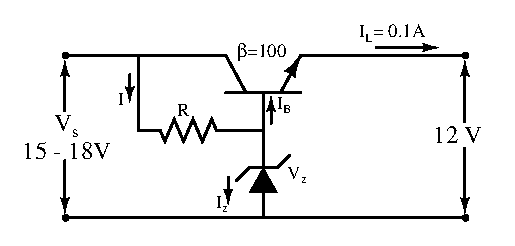
\includegraphics{src/s3/ai/09_303/fig001}\\
Fig. 1.
\end{center}


\item What are the advantages of a bridge rectifier as compared to a full wave
  center-tapped rectifier?

\newpage \again

\item Compare the relative stability of (a) emitter bias and fixed bias circuit, (b)
  emitter bias and voltage divide bias circuits.
\item Explain the essential difference between the RC coupled and direct coupled amplifier.
\item A certain JFET amplifier has g$_\text{m}$ of 4ms, r$_\text{d}$ = 10K$\Omega$ and
  R$_\text{D} = $ 5K$\Omega$. What is the voltage gain? Assume the source resistance to be
  zero.

\markB
\partC

\item \iitem \iitem \iitem Draw the piecewise linear voltampere characteristic of a p-n diode.
\item What is the circuit model for the ON state?
\item The OFF state. \marko{6}
\ene
\item \iitem Derive the expression for I$_\text{C}$ versus  I$_\text{B}$ for a CE
  transistor configuration in the active region.
\item For  I$_\text{B} = 0$, What is  I$_\text{C}$? \marko{4}
\ene \ene
\Or
\item \iitem \iitem  Sketch the circuit of a CS amplifier.
\item Derive the expression for the voltage gain at low frequencies.
\item What is the maximum value of  A$_\text{V}$? \marko{6}
\ene
\item \iitem Sketch the cross section of a p-channel enhancement MOSFET.
\item Show {\em two} circuit symbols for this MOSFET. \marko{4}
\ene \ene\ene

\item \iitem Draw the circuit diagram of full wave rectifiers:
\iitem With center-tap connection and
\item Bridge connection. Explain their working.
\ene
  What is the peak inverse voltage of a diode in each case?
\Or
\item \iitem Draw circuit diagram of transistor shunt regulator. Explain it briefly. \marko{5}
\item A 36V dc voltage is applied through a series resister of 600$\Omega$ to a load
  300$\Omega$ shunted by a zener diode as shown in \mbox{Fig. 2}. if V$_\text{z} = 8$V
  and $\gamma_\text{z} = 10 \Omega$.

  Find (a) dc Load voltage; (b) Power dissipated in the zener and (c) maximum current,
  that a regulator can deliver and still regulate.

\begin{center}
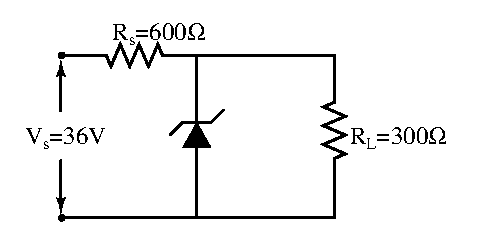
\includegraphics{src/s3/ai/09_303/fig002}\\
Fig. 2.
\end{center}

\ene\ene

\item \iitem \iitem Derive an expression for the stability factor of a fixed bias current. \marko{4}
\item Draw a voltage divider bias circuit and derive an expression for its stability factor.

  \marko{6}
\ene
\Or
\item Derive the expressions for input resistance, output resistance, current gain and voltage gain
  of a common emitter amplifier.
\ene

\item \iitem \iitem What are the biasing schemes available to achieve to achieve the required bias in a 
  JFET? Explain any one of the biasing schemes. \marko{6}
\item A certain JFET has a transconductance (g$_\text{m}$) of 2500$\mu$S. With an external drain
  resistance of 2k$\Omega$. Find the value of ideal voltage gain. \marko{4}
\ene
\Or
\item \iitem Sketch the small signal high frequency circuit of a CS amplifier.
\item Derive the expression for the voltage gain.
\ene\ene

\markC
\ene

